\section{Refleksion}

\begin{frame}
\frametitle{I hvilken kontekst er mobiltelefonen?}
\begin{figure}
\centering
        \begin{subfigure}[b]{0.3\textwidth}
                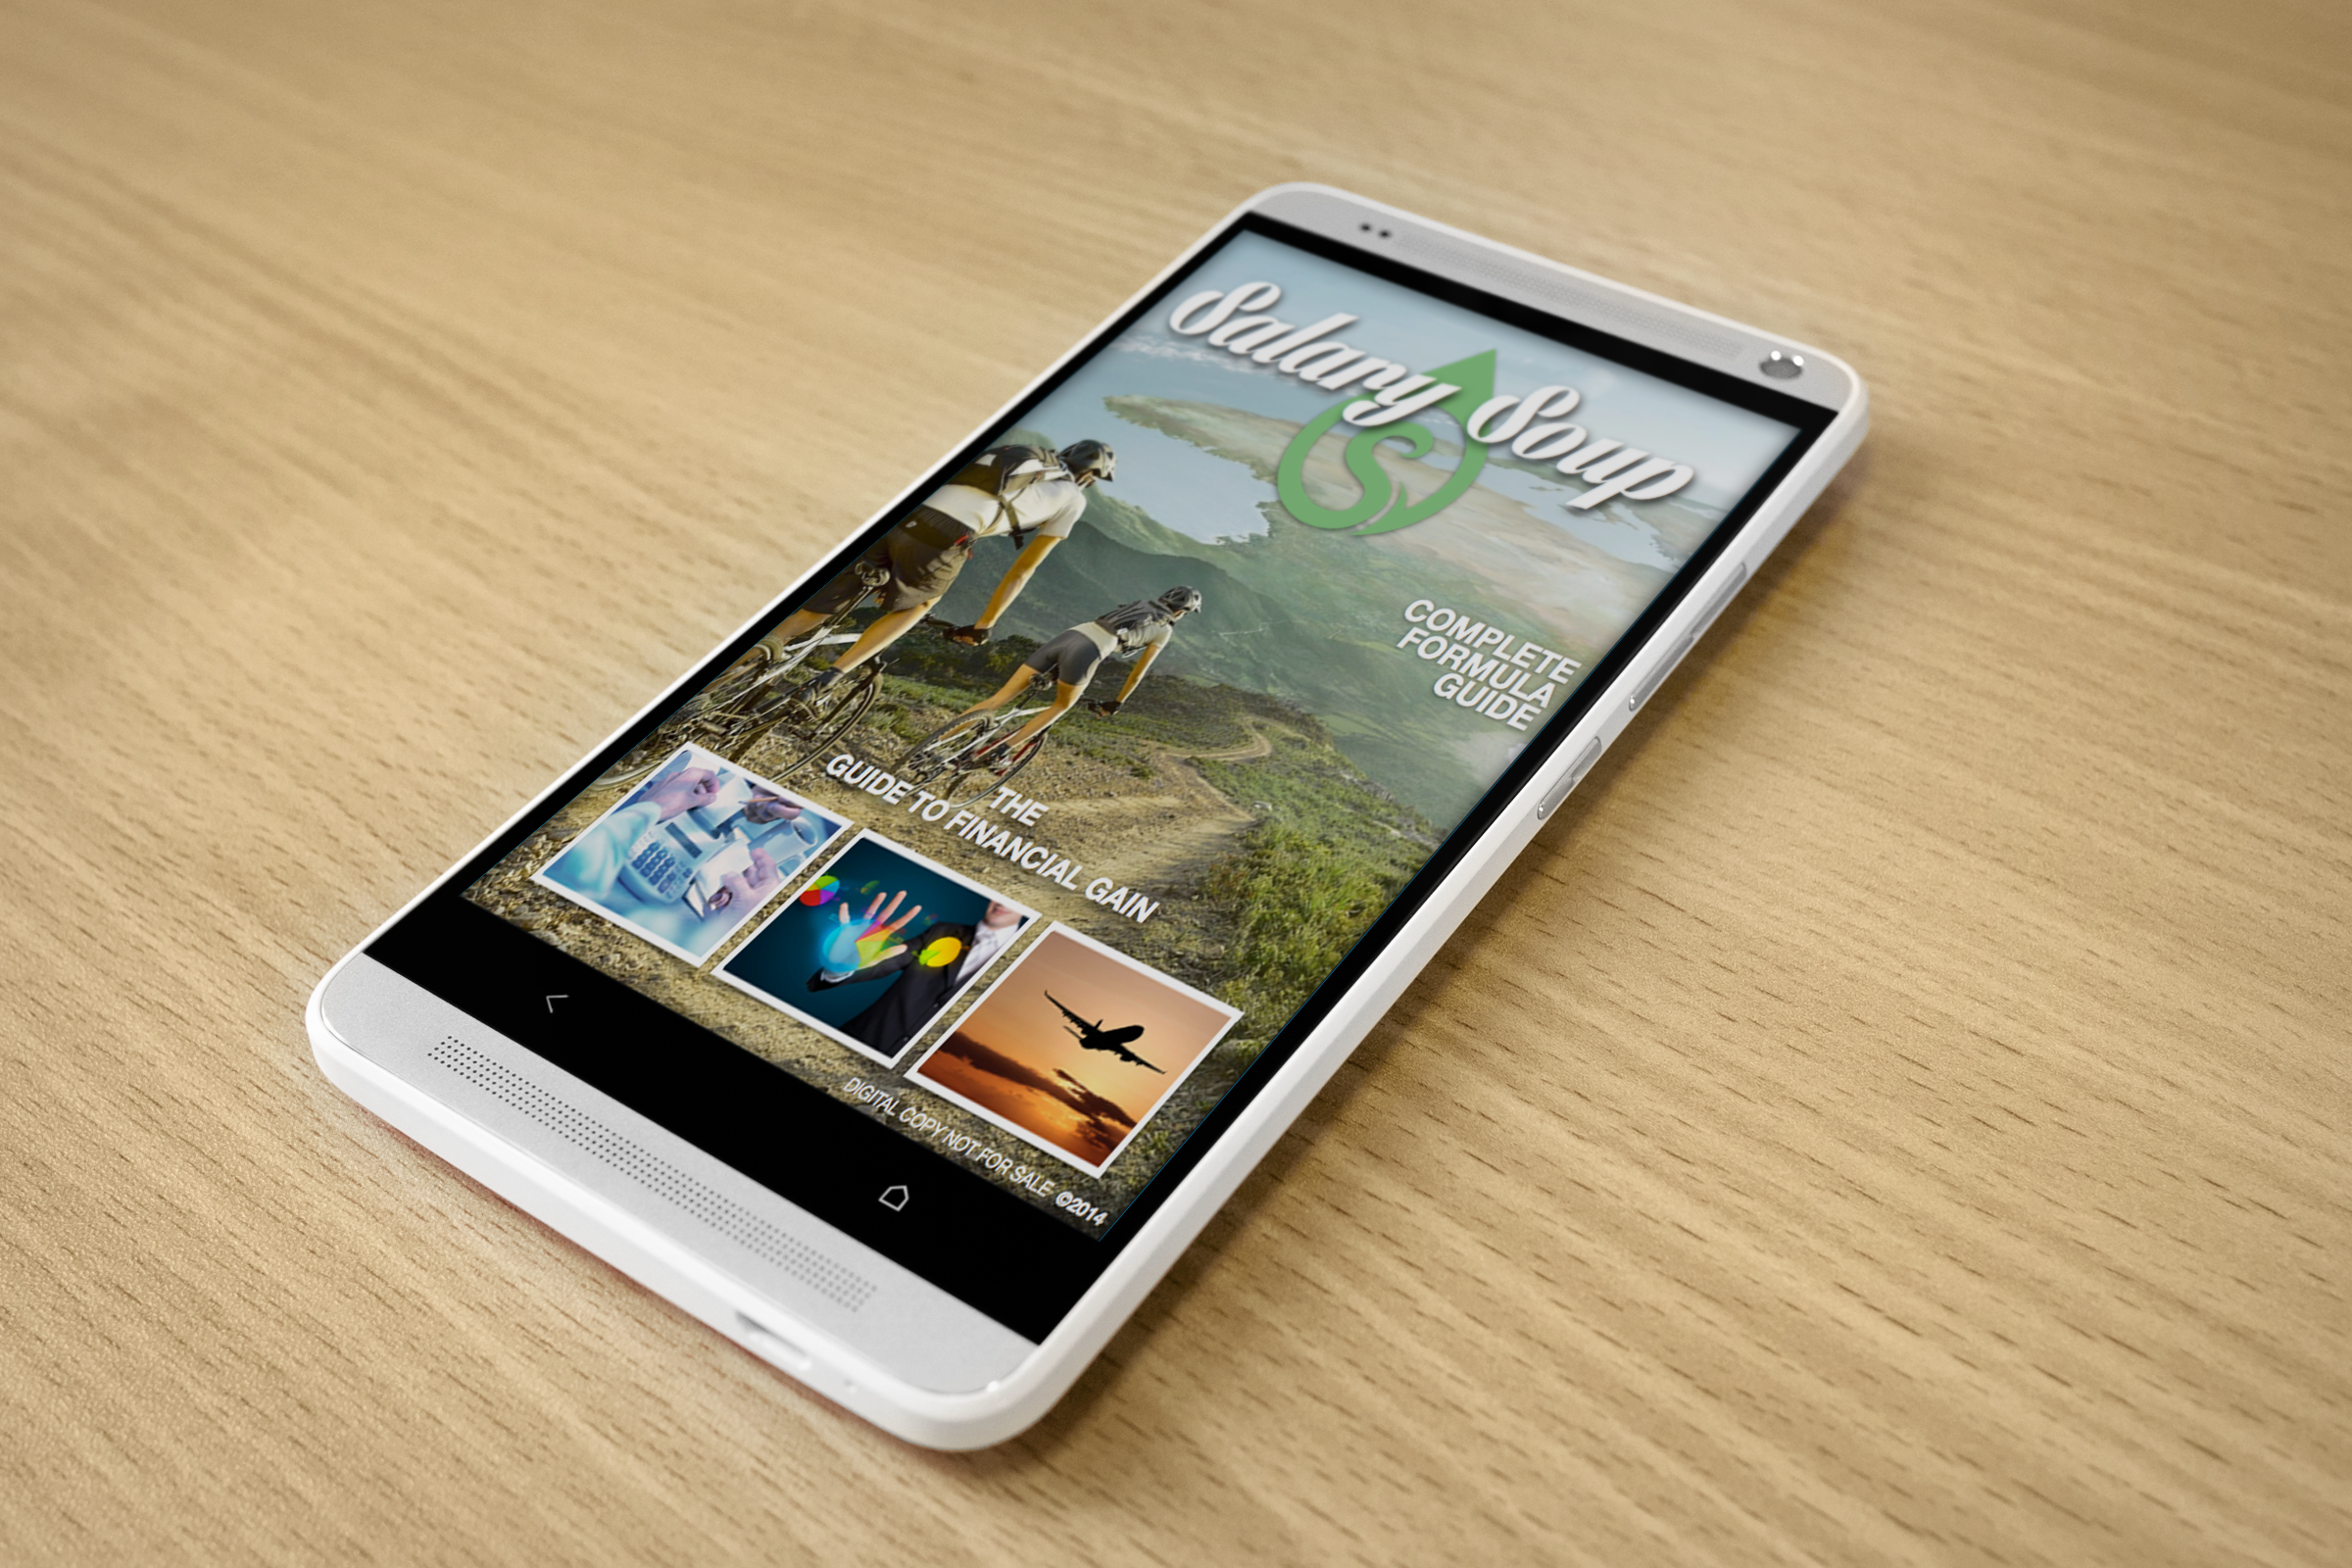
\includegraphics[width=\textwidth]{graphics/smartphone_on_table}
                \caption{Smartphone på et natbord.}
                \label{context:table}
        \end{subfigure}
        ~ %add desired spacing between images, e. g. ~, \quad, \qquad, \hfill etc.
          %(or a blank line to force the subfigure onto a new line)
        \begin{subfigure}[b]{0.3\textwidth}
                \includegraphics[width=\textwidth]{graphics/smartphone_in_purse}
                \caption{Smartphone i en taske.}
                \label{context:purse}
        \end{subfigure}
        ~ %add desired spacing between images, e. g. ~, \quad, \qquad, \hfill etc.
          %(or a blank line to force the subfigure onto a new line)
        \begin{subfigure}[b]{0.3\textwidth}
                \includegraphics[width=\textwidth]{graphics/swimmer}
                \caption{Når man fx er ude at svømme.}
                \label{context:swimmer}
        \end{subfigure}
        \caption{Eksempler på kontekst.}\label{context}
\end{figure}
\end{frame}

\begin{frame}
\frametitle{Notifikationer}
\begin{itemize}
\item På baggrund af fokusgruppeinterviewet er notifikationer en god ide
\item En status for patienten
\item Notifikationer der direkte fortæller om fremgang eller tilbagegang
\item Eller 'refleksionsnotifikationer': Fx at patienten har en dårlig søvnrytmne eller ikke snakker med så mange mennesker som han plejer
\end{itemize}
\end{frame}

\begin{frame}
\frametitle{Huskekort}
\begin{itemize}
\item Hvad er et huskekort?
\item Kan evt. bruges til at sende notifikationer til patienten
\end{itemize}
\end{frame}

\begin{frame}
\frametitle{Dataindsamling}
Pladsmangel kan være et problem, her er nogle mulige løsninger:
\begin{itemize}
\item Gemme data i skyen(Giver ingen komplikationer for arkitekturen)
\item Komprimere data
\item Lavere opdateringshastighed på sensorer
\item Direkte forbindelse mellem moduler, så man ikke behøver at lagre i databasen
\end{itemize}
\end{frame}

\begin{frame}
\frametitle{Databaserettigheder}
\begin{itemize}
\item Alle moduler kan skrive til alle database moduler
\item Mulig løsning: En nøgle kan tilføjes til moduldefinitionen
\item MERE???
\end{itemize}
\end{frame}

\section{Afrunding}
\begin{frame}
\frametitle{Individuelle projekter/moduler}
!?!?!?!?!?!?!?!
\end{frame}
